\documentclass[conference,a4paper]{IEEEtran}
\IEEEoverridecommandlockouts  % conference mode locks out \thanks; needed for the corresponding-author note
\usepackage{graphicx,amsmath,amssymb,booktabs,url,balance}
\usepackage[hidelinks]{hyperref}
\graphicspath{{figs/}}
\renewcommand{\dbltopfraction}{0.93}
\renewcommand{\topfraction}{0.93}
\renewcommand{\textfraction}{0.07}
\renewcommand{\floatpagefraction}{0.72}
\renewcommand{\dblfloatpagefraction}{0.72}
\setcounter{dbltopnumber}{2}\setcounter{topnumber}{3}\setcounter{totalnumber}{4}
\setlength{\textfloatsep}{6pt plus 2pt minus 2pt}
\setlength{\dbltextfloatsep}{8pt plus 2pt minus 2pt}
\setlength{\floatsep}{6pt plus 2pt minus 2pt}
\setlength{\abovedisplayskip}{4pt plus 1pt minus 1pt}
\setlength{\belowdisplayskip}{4pt plus 1pt minus 1pt}
\newcommand{\pos}[1]{\left(#1\right)_+}
\newcommand{\clip}{\operatorname{clip}}
\newcommand{\aeff}{a^{\mathrm{eff}}_{\mathrm{pin},i}}
\begin{document}

\title{Making Way: A Social Force Model Approach to Emergency Vehicle Traffic Dynamics}

\author{\thanks{Corresponding author: sebastian.cubides@tum.de}%
\IEEEauthorblockN{Cristian Sebastian Cubides-Herrera}
\IEEEauthorblockA{Faculty of Automotive Engineering\\Technical University of Munich\\Munich, Germany}
\and
\IEEEauthorblockN{Prof.\ Dr.-Ing.\ Markus Lienkamp}
\IEEEauthorblockA{Faculty of Automotive Engineering\\Technical University of Munich\\Munich, Germany}}

\maketitle

\begin{abstract}
Driving simulators for emergency crews need surrounding traffic that reacts to an approaching emergency vehicle as real drivers do, yet existing emergency vehicle models were built for route planning, traffic-light priority and network analysis and therefore do not reproduce how an individual car gets out of the way. This paper presents a simulation pipeline in which every vehicle is a particle pushed by several behavioural accelerations at once: a perception model decides when each driver reacts, a repulsion from the emergency vehicle and from its expected path decides how strongly, a periodic lane-keeping potential resists the manoeuvre, and a limit taken from a standard car-following model keeps collision avoidance in control. Because the corridor repulsion competes with lane keeping, leaving a lane becomes a threshold phenomenon, known in physics as depinning, whose escape condition and cleared width follow in closed form. Parameters are identified in two stages: ordinary motorway traffic is fitted to drone-recorded trajectories first, and only four repulsion parameters are then fitted to recorded emergency passages. Simulations reproduce detection, yielding and recovery and faster emergency progress in free flow, whereas dense queues remain the main limitation.
\end{abstract}

\begin{IEEEkeywords}
emergency vehicles, social force model, driver yielding behaviour, rescue lane, depinning, parameter identification, driving simulation
\end{IEEEkeywords}

\section{Introduction}
Emergency response underpins the safety of every city, yet the drive to the scene is one of its most dangerous phases. The traffic-related fatality rates of police officers, firefighters and emergency medical technicians have been estimated at 2.5 to 4.8 times the average across all occupations~\cite{hsiao18}, and in one ambulance service 91\,\% of the collisions during responses occurred on runs with warning lights and siren, although such runs made up only 75\,\% of all responses~\cite{custalow04}. Delay also costs lives, since untreated cardiac-arrest survival falls by about 5.5\,\% per minute~\cite{larsen93}.

Training is therefore the lever that emergency organisations control most directly. Although German ambulance drivers have no training standard, simulator training has raised their traffic knowledge and lowered their speed without lengthening response times~\cite{prohn20}, and simulator-trained drivers passed a competency course faster and with fewer penalties~\cite{lindsey08}. Yet a simulator is only as instructive as its traffic.

That traffic is hard to model, because drivers treat an emergency vehicle (EMV), that is, an ambulance, fire engine or police car travelling with warning lights and siren, very differently from other road users and differ widely among themselves. In a driving-simulator study without in-car warnings, only 13 of 33 drivers gave way, eight did not detect the ambulance until it had passed, and those who gave way did so at a mean distance of 23\,m rather than the 84\,m reached when warned~\cite{lidestam20}; likewise, the share of drivers yielding at urban intersections rose from 77.1\,\% to 96.6\,\% once warning signs were installed~\cite{savolainen10}. In Germany, moreover, drivers in slow or stationary motorway traffic must by law open a \emph{rescue lane}, a free passage between the leftmost lane and its neighbour~\cite{stvo11}.

Many methods already represent EMVs, but they pursue other goals: some optimise EMV routes or grant green lights in advance, which is called signal pre-emption~\cite{humagain20,su23}, others plan how communicating vehicles should clear a lane together~\cite{wu20,hannoun19}, and still others estimate EMV trip times and analyse the interactions with surrounding traffic in commercial simulators and real-world scenarios~\cite{cortes23}. Although these approaches serve routing and analysis well, none reproduces how an individual driver perceives the EMV and steers out of its path; indeed, realistic EMV interaction markedly changes the simulated benefit of pre-emption~\cite{kumar24}, and simulators that confine vehicles to discrete lanes need ad hoc rules for sideways motion~\cite{delpiano20}.

This paper models the yielding process explicitly, contributing (i) a social force model separating perception, attempted yielding and constrained movement; (ii) an acceleration combination that keeps safety in control; (iii) a depinning view of lane changing with a closed-form threshold and cleared width; and (iv) a two-stage identification that fits ordinary traffic before the EMV response.

\section{Related Work}
\emph{Network-level models and cooperative clearing.} A systematic review groups EMV support into route optimisation and signal pre-emption and notes that the effect on the remaining traffic is rarely assessed~\cite{humagain20}; multi-agent reinforcement learning has jointly chosen EMV routes and light phases, shortening simulated travel times by up to 42.6\,\%~\cite{su23}. Other work assumes connected vehicles and computes where each should move, through a two-stage optimisation~\cite{wu20} or an integer linear program~\cite{hannoun19}; either way, surrounding vehicles are aggregate flow or perfect cooperators rather than human drivers.

\emph{Microscopic EMV simulation.} Microscopic simulators come closest. SUMO (Simulation of Urban MObility)~\cite{lopez18} gives EMVs a blue-light device that grants special rights and makes traffic form an emergency lane~\cite{biekerwalz18}, yet this lane arises from sideways shifts within each lane rather than lane changes, and vehicles react only within 25\,m by default~\cite{sumodoc}. A recent benchmark couples SUMO with the driving simulator CARLA to control EMV privileges and civilian responses~\cite{zhu26}.

\emph{Modelling foundations.} The Intelligent Driver Model (IDM) describes how a driver accelerates and brakes behind a leader~\cite{treiber00}, and MOBIL (Minimizing Overall Braking Induced by Lane changes) decides whether a lane change is worthwhile and safe~\cite{kesting07}. The social force model expresses pedestrians' intentions as accelerations~\cite{helbing95}, its extension to panicking crowds added body forces~\cite{helbing00}, and a two-dimensional car-following model applies the idea to lateral interaction between vehicles~\cite{delpiano20}. Artificial potential fields push vehicles towards lane centres and away from obstacles in driver assistance~\cite{gerdes01,wolf08}, and physics calls \emph{depinning} the moment an object held by a periodic or random potential breaks free once the driving force exceeds a threshold~\cite{fisher98}. Identification relies on the drone-recorded highD trajectories of German motorways~\cite{krajewski18}, on established calibration practice~\cite{punzo21}, on Latin hypercube sampling, which spreads trial parameter sets evenly over their ranges~\cite{mckay79}, and on the derivative-free Nelder--Mead simplex method~\cite{nelder65}.

\begin{figure*}[t]
\centering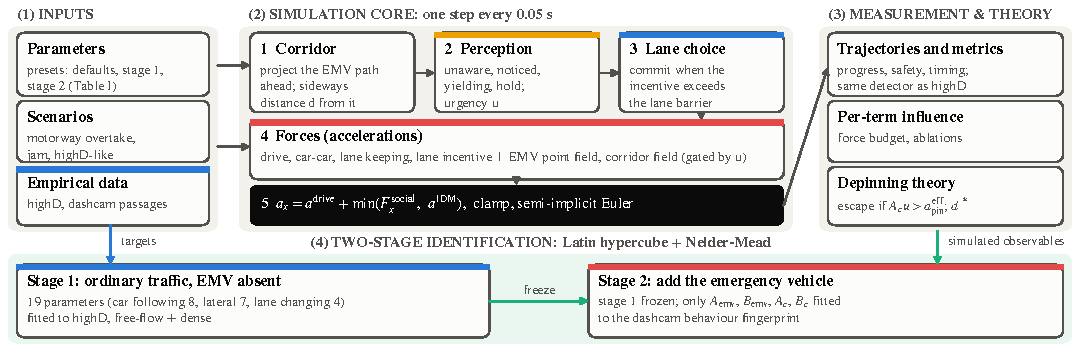
\includegraphics[width=\textwidth]{fig1_pipeline_v4.pdf}
\caption{Pipeline of the framework: (1) inputs; (2) simulation core, applied to all vehicles every 0.05\,s; (3) measurement with the same code as the real data, per-term influence and depinning theory; (4) two-stage identification, first of ordinary traffic without the EMV, then of the four EMV repulsion parameters.}
\label{fig:pipeline}
\end{figure*}

\section{Methodology}
\subsection{Framework overview}
In Fig.~\ref{fig:pipeline}, the inputs~(1) feed the simulation core~(2), which applies five stages to every vehicle at every step, separating \emph{whether} a driver reacts (stages 1--3) from \emph{how} the vehicle moves (stages 4--5). Block~(3) turns trajectories into numbers in three ways. First, metrics of EMV progress, safety and timing use measurement code shared with the real data: one routine detects lane changes in simulated and highD trajectories alike, and simulated traffic is recorded as an EMV-mounted camera would see it, once per second within 50\,m, and labelled yielded, braked, failed to yield or normal by the rules that labelled the real videos, so a mismatch cannot stem from differing definitions. Second, a per-term analysis records each force's share of the acceleration (\emph{force budget}) and the loss of fit when the term is switched off (\emph{ablation}). Third, depinning theory (Section~\ref{sec:depin}) predicts from the parameters whether and how far a vehicle leaves its lane. Block~(4) closes the loop: the deviation between simulated and measured observables (Section~\ref{sec:ident}) drives the search, whose fitted values return to block~(1) as a preset; stage~1 is frozen first, so the EMV terms are fitted on top of ordinary traffic that already matches highD.

\subsection{Inputs and the simulation loop}
The pipeline starts from three inputs: a \emph{parameter set}, whose named variants (\emph{presets}) hold the default and fitted values of Table~\ref{tab:params}; a \emph{scenario}, which builds the road and initial fleet, here a motorway on which the EMV overtakes free-flowing traffic, a crawling jam, or a highD-like motorway with measured lane widths, speeds, truck shares and density; and \emph{empirical data}, namely highD trajectories~\cite{krajewski18} and dashcam videos from EMVs on real emergency runs. Each vehicle $i$ has a position, velocity, length, width and desired speed; the road runs along $x$, and $y$ is the position across it.

The simulation advances in steps of 0.05\,s, and each step passes through the stages of Fig.~\ref{fig:pipeline}. First, the \emph{corridor}, the strip of road the EMV is expected to occupy, is projected ahead along its path over 120 to 260\,m, a length that grows with the EMV speed, and each vehicle's signed sideways distance $d_i$ from the corridor centre line is computed. Second, a perception state machine moves each driver from UNAWARE to NOTICED once the EMV comes within the detection range, $R_{\rm front}=140$\,m when it approaches from behind or 60\,m when it is ahead, to YIELDING after a random reaction delay (median 1\,s), and, once the EMV has passed, to HOLD for a few seconds before merging back; 5\,\% of drivers never react. While yielding, the driver keeps an \emph{urgency} $u_i$ between 0 and 1, which rises as the estimated time until the EMV arrives falls below an anticipation horizon, and in slow traffic also as the siren comes closer, and is zero otherwise; the driver also fixes an escape side $\sigma_i$ ($+1$ left, $-1$ right). Third, ordinary lane changes are decided: a driver held up by a slower leader moves to the next lane when the resulting frustration outweighs the lane-keeping barrier introduced below, and a driver no longer held up returns to the right under the same test, as the keep-right rule demands; a committed driver then receives a constant sideways push $F^{\rm lc}_i$ until the lane marking is crossed. Fourth, the forces are evaluated, and fifth, they are combined and integrated.

\subsection{Force terms}
All forces are per unit mass, i.e.\ accelerations in m/s$^2$.

\emph{Driving force.} Each driver relaxes towards its desired speed through
\begin{equation}
\mathbf a^{\rm drive}_i=\frac{v^0_i\,\hat{\mathbf x}-\mathbf v_i}{\tau},
\label{eq:drive}
\end{equation}
where $v^0_i$ is the desired speed, $\hat{\mathbf x}$ the unit vector along the road, $\mathbf v_i$ the velocity vector and $\tau$ the relaxation time.

\emph{Car--car interaction.} Neighbouring vehicles repel each other, much more strongly along the road than across it:
\begin{equation}
\mathbf F^{\rm cc}_i=\sum_j A_v\,e^{-q_{ij}}\,w_{ij}\,\hat{\mathbf g}_{ij},\qquad q_{ij}=\sqrt{\Big(\frac{g^x_{ij}}{B_x}\Big)^2+\Big(\frac{g^y_{ij}}{B_y}\Big)^2},
\label{eq:cc}
\end{equation}
where the sum runs over the neighbours $j$ of vehicle $i$, $A_v$ is the repulsion strength, $g^x_{ij}$ and $g^y_{ij}$ are the bumper-to-bumper gaps along and across the road, $B_x$ and $B_y$ are the corresponding decay lengths, with $B_x\gg B_y$, $\hat{\mathbf g}_{ij}$ is the unit vector pointing away from $j$, and $w_{ij}$ is a weight that equals 1 for a neighbour straight ahead and falls to the smaller rear weight $\lambda_v$ for one straight behind. A second, short-range copy of this term acts as a body force that stops squeezed vehicles from overlapping. Fig.~\ref{fig:fields}(a) maps the resulting push, whose contours follow the vehicle footprint and reach further ahead than behind.

\begin{figure}[t]
\centering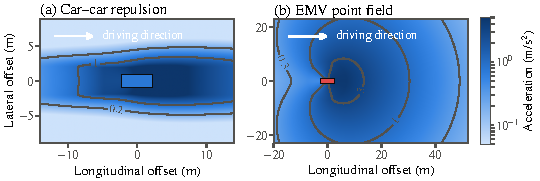
\includegraphics[width=\columnwidth]{fig_fields_v3.pdf}
\caption{Magnitude of (a) the car--car push \eqref{eq:cc} on the blue vehicle from a neighbour at each position and (b) the EMV point field \eqref{eq:ev} on a car at each position around the red EMV, at the stage-2 parameters on one logarithmic scale.}
\label{fig:fields}
\end{figure}

\emph{Lane keeping.} Lane discipline is modelled as a washboard potential, a periodic landscape with valleys at the lane centres and ridges on the markings, whose restoring force is
\begin{align}
F^{\rm lane}_i&=-a^{\rm eff}_{{\rm pin},i}\,\sin\!\Big(\frac{2\pi\,\Delta y_i}{w}\Big),\label{eq:lane}\\
a^{\rm eff}_{{\rm pin},i}&=a_{\rm pin}\Big(\frac{\rho_i}{\rho_{\rm ref}}\Big)^{k_\rho}\big(1-\epsilon\,u_i\big),\label{eq:aeff}
\end{align}
where $\Delta y_i$ is the sideways distance of vehicle $i$ from its lane centre, $w$ the lane width, and $a^{\rm eff}_{{\rm pin},i}$ the effective barrier, i.e.\ the largest restoring acceleration the lane can exert. The barrier grows with the local density $\rho_i$ (vehicles per km in the own lane) relative to a measured reference density $\rho_{\rm ref}$, with exponent $k_\rho$, starting from the base barrier $a_{\rm pin}$, and it is relaxed by urgency through the factor $\epsilon=0.5$. Lateral damping and exponential walls at the road edges complete the lateral behaviour.

\emph{EMV point field.} Drivers who are yielding or holding are pushed away from the EMV itself by
\begin{equation}
\mathbf F^{\rm EMV}_i=A_{\rm emv}\,e^{-\ell_i/B_{\rm emv}}\,w^{\rm EMV}_i\,\hat{\mathbf n}_i,
\label{eq:ev}
\end{equation}
where $\ell_i$ is the distance between the EMV and car $i$ (minus a small size offset), $A_{\rm emv}$ and $B_{\rm emv}$ are the strength and range of the field, $\hat{\mathbf n}_i$ is the unit vector from the EMV to the car, and $w^{\rm EMV}_i$ is a weight that equals 1 straight ahead of the EMV and 0.1 straight behind it. As Fig.~\ref{fig:fields}(b) shows, this field reaches much further than the car--car push but fades astern, so it clears the space just ahead of the EMV.

\emph{Corridor field.} The key term repels vehicles from the projected corridor rather than from the EMV, so that drivers far along its path can react in time:
\begin{equation}
F^{\rm corr}_i=A_c\,\exp\!\Big(-\frac{\max\big(|d_i|-w^{\rm need}_i,\,0\big)}{B_c}\Big)\,u_i\,\sigma_i,
\label{eq:corr}
\end{equation}
where $A_c$ is the corridor strength, $d_i$ the sideways distance from the corridor centre line, $w^{\rm need}_i$ the required clearance (half the summed widths of the EMV and the car plus a 0.5\,m margin), $B_c$ the decay length beyond that clearance, $u_i$ the urgency and $\sigma_i$ the escape side. In addition, a car that still blocks the corridor is slowed towards 82\,\% of its desired speed, so that it can drop into a gap in the next lane instead of pacing the EMV, and the field fades out over the last 30\,m of the corridor.

\subsection{Acceleration decomposition}
The forces are not simply added. Along the road, all behavioural forces are merged and then bounded by the safety demand of the IDM,
\begin{align}
a_{x,i}&=a^{\rm drive}_{x,i}+\min\!\big(F^{\rm social}_{x,i},\ a^{\rm IDM}_i\big),\label{eq:ax}\\
a_{y,i}&=a^{\rm drive}_{y,i}+F^{\rm lane}_i+F^{\rm corr}_i+F^{\rm lc}_i+F^{\rm cc}_{y,i}+F^{\rm EMV}_{y,i},\label{eq:ay}
\end{align}
where the subscripts $x$ and $y$ denote the components along and across the road, $F^{\rm social}_{x,i}$ is the sum of the car--car, EMV and corridor-slowdown forces along the road, and $a^{\rm IDM}_i$ is the deceleration (a negative acceleration) that the IDM requires to keep a safe gap to the vehicle ahead. The minimum in \eqref{eq:ax} lets $a^{\rm IDM}_i$ override every behavioural term whenever a leader is close, and several mild braking terms can never add up to harder braking than safety requires. Across the road, the lane barrier, road walls and body force already oppose unsafe motion. Accelerations and lateral speeds are capped at comfortable values, and states are advanced with a semi-implicit Euler scheme, which remains stable for stiff short-range forces.

\subsection{Depinning: when and how far a vehicle leaves its lane}
\label{sec:depin}
Consider a yielding vehicle that still blocks the corridor, so that \eqref{eq:corr} pushes it sideways with the constant acceleration $A_c u_i$. According to \eqref{eq:lane}, the lane can hold it back with at most $a^{\rm eff}_{{\rm pin},i}$, reached halfway between the lane centre and the marking, because a sine never exceeds one. A weaker push only shifts the vehicle within its lane; a stronger one leaves no resting position and carries it into the next lane. The escape condition is therefore
\begin{equation}
A_c\,u_i>a^{\rm eff}_{{\rm pin},i},
\label{eq:escape}
\end{equation}
which is exactly the depinning of a driven particle from a periodic potential~\cite{fisher98}. Beyond the required clearance, the push \eqref{eq:corr} decays exponentially, and the vehicle stops where it equals the maximum restoring force, at the \emph{cleared half-width}
\begin{equation}
d^*=w^{\rm need}_i+B_c\,\ln\!\frac{A_c\,u_i}{a^{\rm eff}_{{\rm pin},i}},
\label{eq:dstar}
\end{equation}
the distance from the corridor centre line at which a yielding vehicle settles. Both results depend on the corridor and the lane only through the \emph{control ratio} $x=A_cu_i/a^{\rm eff}_{{\rm pin},i}$: the corridor opens for $x>1$, and $d^*$ grows with $\ln x$, so denser traffic, which raises the barrier, clears a narrower passage. Ordinary lane changes cross the same barrier, so a faster follower and an EMV move a vehicle sideways through one mechanism of different strength and range.

\begin{table}[t]
\caption{Tunable parameters; bold values were fitted in that stage, others are inherited.}
\label{tab:params}
\centering\scriptsize
\setlength{\tabcolsep}{2.6pt}\renewcommand{\arraystretch}{0.8}
\begin{tabular}{@{}lllrrr@{}}
\toprule
Symbol & Meaning & Unit & Default & Stage 1 & Stage 2\\
\midrule
\csname @@input\endcsname param_table_v3.tex
\bottomrule
\end{tabular}
\end{table}

\begin{table}[t]
\caption{Yielding versus no yielding (mean $\pm$ standard deviation over runs).}
\label{tab:res}
\centering\footnotesize\setlength{\tabcolsep}{3pt}
\begin{tabular}{@{}llcc@{}}
\toprule
Scenario & Traffic & EMV speed ratio & Clearance (m)\\
\midrule
highD-like & yields & $0.96\pm0.04$ & $113\pm25$\\
 & no yield & $0.90\pm0.05$ & $83\pm20$\\
Overtake & yields & $0.89\pm0.04$ & $49\pm8$\\
 & no yield & $0.82\pm0.04$ & $38\pm8$\\
Jam (5 runs) & yields & $0.70\pm0.03$ & $8.3\pm0.5$\\
 & no yield & $0.29\pm0.03$ & $3.8\pm0.5$\\
\bottomrule
\end{tabular}
\end{table}

\subsection{Identification}
\label{sec:ident}
Simulated observables such as EMV progress (mean over desired speed), free distance ahead of the EMV, yield-onset distance, headways and lane-change kinematics are compared with their measured values through the weighted deviation
\begin{equation}
D(\boldsymbol\theta)=\frac{\sum_k \omega_k\,|m_k(\boldsymbol\theta)-\hat m_k|/\delta_k}{\sum_k\omega_k},
\label{eq:loss}
\end{equation}
where $\boldsymbol\theta$ is the vector of parameters being fitted, $m_k(\boldsymbol\theta)$ the $k$-th simulated observable, $\hat m_k$ its measured value, $\delta_k$ a typical scale that makes the deviation dimensionless, and $\omega_k$ its weight.

The fit proceeds in two stages. In \emph{stage~1}, the EMV is removed, so that it cannot cause any lane change, and nineteen parameters describing car following, lateral behaviour and lane changing are fitted to highD traffic in free-flowing and dense conditions, with congested traffic and some recording locations held back for validation. In \emph{stage~2}, these parameters are frozen and only $A_{\rm emv}$, $B_{\rm emv}$, $A_c$ and $B_c$ are fitted to statistics pooled over five dashcam videos (the shares of vehicles that yielded, braked or failed to yield, the onset distance and the lateral speed), plus penalties for unsafe or uncomfortable driving. Both stages explore the parameter space with Latin hypercube sampling~\cite{mckay79} and refine the best candidates with Nelder--Mead~\cite{nelder65,punzo21}.

\begin{figure*}[t]
\centering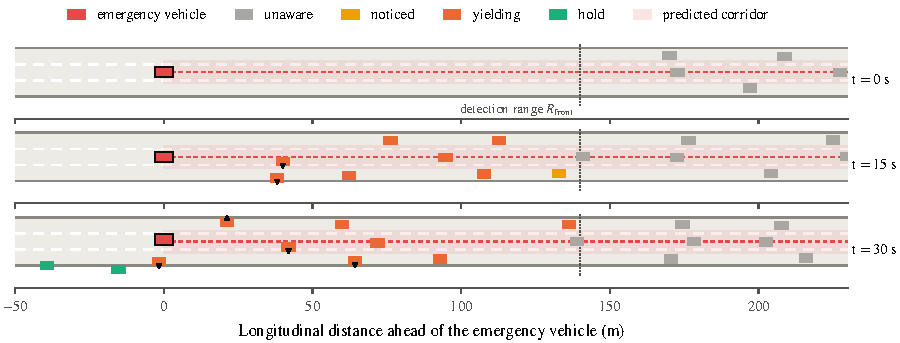
\includegraphics[width=0.80\textwidth]{fig2_snapshots.pdf}
\caption{Detection and yielding (overtaking, 22 vehicles per km per lane; frame moving with the EMV, lateral distances exaggerated): all 137 vehicles unaware at $t=0$\,s; seven yielding and one noticing at 15\,s; eight yielding and two holding at 30\,s.}
\label{fig:snap}
\end{figure*}

\section{Implementation}
The framework is a Python package relying only on NumPy and Matplotlib; it evaluates each force for all vehicles at once, implements its own optimisers, and logs the parameters, metrics and outputs of every experiment. One update of 113 vehicles takes 2.6\,ms on a single processor core, fast enough for real-time use around a trainee.

\emph{Parameter tuning.} Table~\ref{tab:params} lists the 25 tunable parameters. Stage~1 reached a deviation of 1.524, against 4.689 for an earlier single-stage fit scored with an EMV present and 5.327 for the defaults, and it scores 1.53 against 3.95 on held-out locations. Stage~2 reached 0.942 on the calibration runs and 1.068 on runs started from different random initial conditions.

\section{Results}
\label{sec:results}
All simulations use the stage-2 preset; Table~\ref{tab:res} pairs 10 random initial conditions (5 in the jam) with identical runs without yielding, and Fig.~\ref{fig:bow} pools 40 of them.

\emph{Detection and yielding.} Fig.~\ref{fig:snap} shows the perception stage at work, and over 40 runs and 736 vehicles yielding begins a median of 85.7\,m ahead of the EMV, with 10th and 90th percentiles of 42.0 and 126.0\,m (Fig.~\ref{fig:bow}, right). Since the mean urgency is zero beyond about 150\,m and only 0.49 at 45\,m, the sideways response concentrates in the last tens of metres before the EMV (Fig.~\ref{fig:bow}, left). Drivers thus notice the EMV long before they move, so a trainee must anticipate when, and to which side, vehicles still in their lane will move. The median onset is close to the 84\,m of warned rather than the 23\,m of unwarned drivers~\cite{lidestam20}, although the distances are defined differently, so the detection range describes an attentive population.

\begin{figure}[t]
\centering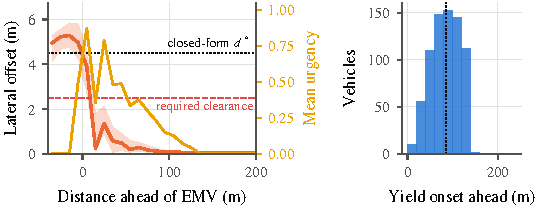
\includegraphics[width=\columnwidth]{fig3_bowwave_v3.pdf}
\caption{Bow wave (overtaking, 40 runs): sideways distance from the corridor centre line of initially blocking vehicles, and mean urgency, against distance ahead of the EMV (left); yield-onset distances (right).}
\label{fig:bow}
\end{figure}

\emph{Effect on the EMV.} As Table~\ref{tab:res} shows, on the free-flowing highD-like motorway the EMV reaches 96\,\% of its desired speed instead of 90\,\% and the free distance ahead of it grows from 83 to 113\,m, and in the denser overtaking scenario the speed ratio rises from 0.82 to 0.89. In the jam, yielding lifts EMV progress from 0.29 to 0.70. The benefit thus grows with density, from 6--7 percentage points in moving traffic to 41 in the jam, where an EMV without a rescue lane crawls at under a third of its desired speed; in free flow it appears mainly as a 36\,\% longer free distance, i.e.\ more reaction time for the EMV driver. Yielding matters most where the model is least reliable, however: the stiff stage-1 lane discipline produces body contact in the queue, so the jam gain is likely optimistic.

\begin{figure}[t]
\centering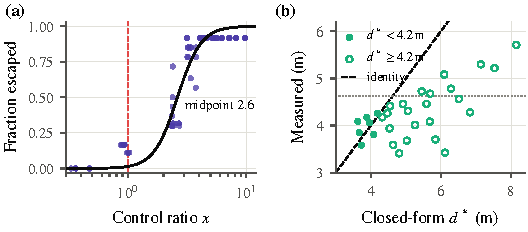
\includegraphics[width=\columnwidth]{fig4_depinning.pdf}
\caption{Depinning in 72 simulations varying $A_c$, $B_c$ and $a_{\rm pin}$ with density dependence switched off ($k_\rho=0$): (a) share of blocking vehicles that left the corridor against the control ratio $x$ (mean urgency), with a fitted logistic curve; (b) measured cleared half-width against $d^*$ \eqref{eq:dstar}, saturation dotted.}
\label{fig:depin}
\end{figure}

\emph{Per-term influence.} While drivers yield, the corridor field supplies 27--29\,\% of their lateral acceleration, the EMV point field only 6--8\,\%. Removing the corridor field at the stage-2 fit raises $D$ by 0.661, almost as much as removing every EMV response (0.683), and cuts the clearance ahead of the EMV from 118 to 68\,m, whereas the point field costs 0.088: the corridor, not the EMV itself, forms the rescue lane. Anticipating the EMV's path, not reacting to its proximity as with SUMO's default 25\,m range~\cite{sumodoc}, is what opens a lane in time. Removing the urgency relief of lane discipline costs 0.260, three times the point field.

\emph{Depinning.} Fig.~\ref{fig:depin} confirms that corridor formation is a sharp transition in the control ratio $x$: below $x=1$ only 7\,\% of blocking vehicles leave, and the fitted curve reaches its midpoint at $x=2.6$, above the idealised value of one because neighbours and reaction delays oppose escape. Where \eqref{eq:dstar} predicts less than 4.2\,m, the measured half-width follows it with a root-mean-square error of 0.25\,m, beyond which it saturates near 4.6\,m, a limit set by the next lane and the road edge. At the overtaking density the stage-2 values give $x=2.0$, below the midpoint, which is consistent with the late clearing in Fig.~\ref{fig:bow}. Corridor formation is thus nearly all-or-nothing, and the fitted model sits on the steep part of the curve, where a modest rise in density can switch clearing off, so parameters fitted at one density need not transfer to another. Conversely, $x$ is one interpretable setting for how compliant a training scenario is.

\section{Limitations and Further Steps}
\emph{Data.} Stage~2 rests on five ambulance dashcam videos observed at 1\,Hz within 50\,m ahead, which leaves more distant drivers unconstrained, and its out-of-sample deviation of 1.068 exceeds the 0.725 spread between videos. Stage~1 deviations (1.50 free flow, 0.84 dense) are two to three times highD's own spread between carriageways (0.49, 0.39), car following is harsher than observed, and perception parameters are set by hand.

\emph{Dense traffic and scope.} Jam queues still produce body contact (183 frames with overlaps in five runs); congested traffic (37.8 vehicles per km per lane) spans only two highD carriageways, so $k_\rho$ is weakly identified. Only motorways are modelled, and $a_{\rm pin}$ sets both lane-change rate and duration.

\emph{Further steps.} The EMV block and the perception parameters will be fitted across densities with more, longer-range recordings; the lane-change threshold will be separated from the lane barrier and overlap in queues prevented; and the model will be extended to intersections and coupled to the driving simulator (113 vehicles use 16\,\% of a 60\,Hz frame) to test its training effect.

\section{Conclusions}
The presented pipeline simulates yielding to an EMV as a continuous, perception-gated physical process; its acceleration decomposition keeps the safety demand of a car-following model in control, and its lane-keeping potential turns lane changing into a depinning transition with a closed-form threshold, a cleared width and one mechanism shared by ordinary and emergency lane changes. The results imply that anticipating the EMV's path forms the rescue lane, that yielding pays off most in dense traffic, and that corridors form sharply above a threshold.

%\balance
\raggedbottom
\vspace{5pt}
\noindent\begin{minipage}{\columnwidth}
\section*{Acknowledgment}
\indent This work was supported by the German Federal Ministry of Research, Technology and Space (BMFTR) under grant number 13N17326 within the call `KMU-innovativ: Forschung f\"ur die zivile Sicherheit' of the Federal Government's programme `Forschung f\"ur die zivile Sicherheit 2018 bis 2023' (\mbox{www.sifo.de}), as part of the joint project `Einsatzfahrt-Simulator f\"ur das Ehrenamt (EfaSim)', sub-project `Prozedurale Generierung und Integration von Umgebungsinformationen in die digitale Ausbildung', at the Technical University of Munich.

\vspace{2pt}
\centering
\raisebox{-0.5\height}{
\includegraphics[height=0.32in]{logo_bmftr.png}}\hspace{0.35in}
\raisebox{-0.5\height}{
\includegraphics[height=0.20in]{logo_sifo.jpg}}
\end{minipage}

\vspace{4pt}
\noindent \emph{Use of AI tools:} generative AI tools were used to draft and revise sections of the manuscript and to support the analysis code and figure generation. All AI-assisted output was checked and edited by the authors, who take full responsibility for the content of this paper.

\begin{thebibliography}{99}
\scriptsize
\bibitem{hsiao18} H.~Hsiao, J.~Chang, and P.~Simeonov, ``Preventing emergency vehicle crashes: Status and challenges of human factors issues,'' \emph{Human Factors}, vol.~60, no.~7, pp.~1048--1072, 2018.
\bibitem{custalow04} C.~B. Custalow and C.~S. Gravitz, ``Emergency medical vehicle collisions and potential for preventive intervention,'' \emph{Prehospital Emergency Care}, vol.~8, no.~2, pp.~175--184, 2004.
\bibitem{larsen93} M.~P. Larsen, M.~S. Eisenberg, R.~O. Cummins, and A.~P. Hallstrom, ``Predicting survival from out-of-hospital cardiac arrest: A graphic model,'' \emph{Annals of Emergency Medicine}, vol.~22, no.~11, pp.~1652--1658, 1993.
\bibitem{prohn20} M.~J. Prohn and B.~Herbig, ``Evaluating the effects of a simulator-based training on knowledge, attitudes and driving profiles of German ambulance drivers,'' \emph{Accident Analysis \& Prevention}, vol.~138, art.~105466, 2020.
\bibitem{lindsey08} J.~T. Lindsey and A.~E. Barron, ``Effects of simulation on emergency vehicle drivers' competency in training,'' \emph{Prehospital and Disaster Medicine}, vol.~23, no.~4, pp.~361--368, 2008.
\bibitem{lidestam20} B.~Lidestam, B.~Thorslund, H.~Selander, D.~N\"asman, and J.~Dahlman, ``In-car warnings of emergency vehicles approaching: Effects on car drivers' propensity to give way,'' \emph{Frontiers in Sustainable Cities}, vol.~2, art.~19, 2020.
\bibitem{savolainen10} P.~T. Savolainen, T.~K. Datta, I.~Ghosh, and T.~J. Gates, ``Effects of dynamically activated emergency vehicle warning sign on driver behavior at urban intersections,'' \emph{Transportation Research Record}, vol.~2149, pp.~77--83, 2010.
\bibitem{stvo11} ``Stra{\ss}enverkehrs-Ordnung (StVO), {\S}\,11 Besondere Verkehrslagen, Abs.~2,'' Federal Ministry of Justice, Germany. [Online]. Available: \url{https://www.gesetze-im-internet.de/stvo_2013/__11.html}
\bibitem{humagain20} S.~Humagain, R.~Sinha, E.~Lai, and P.~Ranjitkar, ``A systematic review of route optimisation and pre-emption methods for emergency vehicles,'' \emph{Transport Reviews}, vol.~40, no.~1, pp.~35--53, 2020.
\bibitem{su23} H.~Su, Y.~D. Zhong, J.~Y.~J. Chow, B.~Dey, and L.~Jin, ``EMVLight: A multi-agent reinforcement learning framework for an emergency vehicle decentralized routing and traffic signal control system,'' \emph{Transportation Research Part C}, vol.~146, art.~103955, 2023.
\bibitem{wu20} J.~Wu, B.~Kulcs\'ar, S.~Ahn, and X.~Qu, ``Emergency vehicle lane pre-clearing: From microscopic cooperation to routing decision making,'' \emph{Transportation Research Part B}, vol.~141, pp.~223--239, 2020.
\bibitem{hannoun19} G.~J. Hannoun, P.~Murray-Tuite, K.~Heaslip, and T.~Chantem, ``Facilitating emergency response vehicles' movement through a road segment in a connected vehicle environment,'' \emph{IEEE Transactions on Intelligent Transportation Systems}, vol.~20, no.~9, pp.~3546--3557, 2019.
\bibitem{cortes23} C.~E. Cort\'es and B.~Stefoni, ``Trajectory simulation of emergency vehicles and interactions with surrounding traffic,'' \emph{Journal of Advanced Transportation}, vol.~2023, art.~5995950, 2023.
\bibitem{kumar24} G.~N. Suresh~Kumar, M.~Hunter, and A.~Guin, ``Enhancing driver behavior models in response to emergency vehicles,'' in \emph{Proc. Winter Simulation Conference (WSC)}, 2024, pp.~1410--1421.
\bibitem{lopez18} P.~A. Lopez \emph{et al.}, ``Microscopic traffic simulation using SUMO,'' in \emph{Proc. IEEE ITSC}, 2018, pp.~2575--2582.
\bibitem{biekerwalz18} L.~Bieker-Walz, M.~Behrisch, and M.~Junghans, ``Analysis of the traffic behavior of emergency vehicles in a microscopic traffic simulation,'' in \emph{SUMO 2018}, EPiC Series in Engineering, vol.~2, pp.~1--13, 2018.
\bibitem{sumodoc} Eclipse SUMO, ``Emergency vehicles,'' SUMO Documentation. [Online]. Available: \url{https://sumo.dlr.de/docs/Simulation/Emergency.html}
\bibitem{zhu26} Y.~Zhu, T.~Zhao, H.~Leng, F.~Zuo, T.~Li, and Z.~Bian, ``SIREN-Bench: Behavior-driven generation and evaluation of emergency-vehicle interactions,'' 2026, arXiv:2608.24094.
\bibitem{treiber00} M.~Treiber, A.~Hennecke, and D.~Helbing, ``Congested traffic states in empirical observations and microscopic simulations,'' \emph{Physical Review E}, vol.~62, no.~2, pp.~1805--1824, 2000.
\bibitem{kesting07} A.~Kesting, M.~Treiber, and D.~Helbing, ``General lane-changing model MOBIL for car-following models,'' \emph{Transportation Research Record}, vol.~1999, pp.~86--94, 2007.
\bibitem{helbing95} D.~Helbing and P.~Moln\'ar, ``Social force model for pedestrian dynamics,'' \emph{Physical Review E}, vol.~51, no.~5, pp.~4282--4286, 1995.
\bibitem{helbing00} D.~Helbing, I.~Farkas, and T.~Vicsek, ``Simulating dynamical features of escape panic,'' \emph{Nature}, vol.~407, pp.~487--490, 2000.
\bibitem{delpiano20} R.~Delpiano, J.~C. Herrera, J.~Laval, and J.~E. Coeymans, ``A two-dimensional car-following model for two-dimensional traffic flow problems,'' \emph{Transportation Research Part C}, vol.~114, pp.~504--516, 2020.
\bibitem{gerdes01} J.~C. Gerdes and E.~J. Rossetter, ``A unified approach to driver assistance systems based on artificial potential fields,'' \emph{Journal of Dynamic Systems, Measurement, and Control}, vol.~123, no.~3, pp.~431--438, 2001.
\bibitem{wolf08} M.~T. Wolf and J.~W. Burdick, ``Artificial potential functions for highway driving with collision avoidance,'' in \emph{Proc. IEEE ICRA}, 2008, pp.~3731--3736.
\bibitem{fisher98} D.~S. Fisher, ``Collective transport in random media: From superconductors to earthquakes,'' \emph{Physics Reports}, vol.~301, no.~1--3, pp.~113--150, 1998.
\bibitem{krajewski18} R.~Krajewski, J.~Bock, L.~Kloeker, and L.~Eckstein, ``The highD dataset: A drone dataset of naturalistic vehicle trajectories on German highways for validation of highly automated driving systems,'' in \emph{Proc. IEEE ITSC}, 2018, pp.~2118--2125.
\bibitem{punzo21} V.~Punzo, Z.~Zheng, and M.~Montanino, ``About calibration of car-following dynamics of automated and human-driven vehicles: Methodology, guidelines and codes,'' \emph{Transportation Research Part C}, vol.~128, art.~103165, 2021.
\bibitem{mckay79} M.~D. McKay, R.~J. Beckman, and W.~J. Conover, ``A comparison of three methods for selecting values of input variables in the analysis of output from a computer code,'' \emph{Technometrics}, vol.~21, no.~2, pp.~239--245, 1979.
\bibitem{nelder65} J.~A. Nelder and R.~Mead, ``A simplex method for function minimization,'' \emph{The Computer Journal}, vol.~7, no.~4, pp.~308--313, 1965.
\end{thebibliography}
\end{document}
